% =====================================================
% Fig. 7 : CFET(Complementary FET)垂直積層構造 断面図
% =====================================================
\begin{figure}[t]
  \centering
  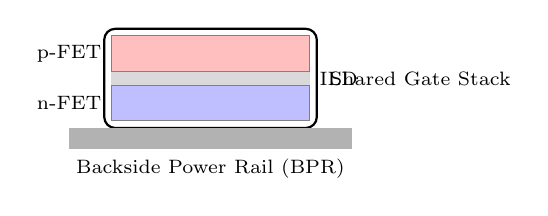
\begin{tikzpicture}[scale=0.9, every node/.style={font=\scriptsize}]
    % bottom n-FET
    \fill[blue!25] (0.6,0.4) rectangle (3.4,0.9);
    \draw[black!50] (0.6,0.4) rectangle (3.4,0.9);
    \node[left] at (0.6,0.65) {n-FET};

    % isolation (ILD)
    \fill[gray!30] (0.6,0.9) rectangle (3.4,1.1);
    \node[right] at (3.4,1.0) {ILD};

    % top p-FET
    \fill[red!25] (0.6,1.1) rectangle (3.4,1.6);
    \draw[black!50] (0.6,1.1) rectangle (3.4,1.6);
    \node[left] at (0.6,1.35) {p-FET};

    % gate stack
    \draw[thick,rounded corners] (0.5,0.3) rectangle (3.5,1.7);
    \node[right] at (3.55,1.0) {Shared Gate Stack};

    % backside power rail (BPR)
    \fill[gray!60] (0,0) rectangle (4,0.3);
    \node[below] at (2,0) {Backside Power Rail (BPR)};
  \end{tikzpicture}

  \caption{CFET構造の垂直積層模式図(n/pスタックおよびBPRを示す)\\
  \footnotesize Schematic vertical stack of CFET showing n/p layers and backside power rail.}
  \label{fig:cfet_cross}
\end{figure}
